\documentclass[a4paper,12pt]{report}

\usepackage{alltt, fancyvrb, url}
\usepackage{graphicx}
\usepackage[utf8]{inputenc}
\usepackage{float}
\usepackage{hyperref}

% Questo commentalo se vuoi scrivere in inglese.
\usepackage[italian]{babel}

\usepackage[italian]{cleveref}

\title{Relazione Assignment-01 \\ per l'esame \\ ``Programmazione Concorrente e distribuita''}
\author{Rattini Emiliano\\Giosuè Giocondo Mainardi}

\date{\today}


\begin{document}

\maketitle

\tableofcontents

\chapter{Analisi}
% A brief analsysis of the problem, focusing in particular aspects that are relevant from concurrent point of view.
Il modello di simulazione dei boid, formulato da Craig Reynolds nel 1986, rappresenta un sistema multi-agente in cui 
entità autonome (boid) si muovono in uno spazio condiviso, modificando la propria traiettoria in funzione dei boid 
circostanti e di parametri predefiniti.

Dal punto di vista computazionale, l'algoritmo richiede l'aggiornamento sincronizzato delle velocità di ciascun boid 
in base alle posizioni correnti dei vicini, seguito dall'aggiornamento delle posizioni secondo le nuove velocità 
calcolate, per poi infine renderizzare lo stato aggiornato tramite l'interfaccia grafica.

In ottica di ottimizzazione delle prestazioni tramite programmazione concorrente, emerge l'opportunità di distribuire 
il carico computazionale tra più unità di elaborazione. Tale distribuzione deve tuttavia preservare la correttezza 
dell'algoritmo, garantendo che l'aggiornamento delle velocità preceda sempre quello delle posizioni, e che la 
visualizzazione avvenga solo a computazione completata.

Le tre implementazioni concorrenti sviluppate (multithreading tradizionale, framework Executor e virtual threads) 
presentano approcci distinti alla parallelizzazione, pur mantenendo invariata la semantica del problema.

\chapter{Design}
% A description of the adopted design, the strategy and architecture.
Il design implementato presenta una struttura architetturale modulare e flessibile, centrata attorno all'interfaccia `BoidsSimulator` che definisce il contratto fondamentale per tutte le implementazioni. Questa interfaccia è parzialmente realizzata dalla classe astratta `AbstractBoidsSimulator`, che fornisce l'implementazione comune e definisce due metodi astratti: `init()` per l'inizializzazione e `clear()` per la pulizia delle risorse.

Da questa classe astratta derivano le implementazioni concrete:
\begin{itemize}
    \item `BoidsSimulator`: implementazione sequenziale di riferimento
    \item `BoidsSimulatorPlatform`: versione concorrente basata su platform threads
    \item `BoidsSimulatorExecutor`: versione che utilizza il framework Executor con approccio task-based
    \item `BoidsSimulatorVirtual`: versione che sfrutta i virtual threads introdotti in Java 19, in realtà questa estende direttamente `BoidsSimulatorPlatform`, in quanto condivide parte dei meccanismi di sincronizzazione
\end{itemize}

\section{Modifiche generali}

L'architettura è stata progettata per massimizzare la reattività dell'interfaccia utente: le operazioni di avvio, interruzione e ripresa della simulazione vengono gestite attraverso variabili di stato condivise, evitando operazioni bloccanti nel ciclo di rendering.

Una modifica architetturale significativa è stata la migrazione della generazione iniziale dei boid dalla View al Controller. Questo cambio ha migliorato la reattività dell'interfaccia utente, evitando di sovraccaricare l'Event Dispatch Thread (EDT) di Swing con operazioni computazionalmente intensive.

Questo approccio permette di eseguire la creazione dei boid sul main thread, lasciando l'EDT libero di gestire esclusivamente gli eventi dell'interfaccia grafica, garantendo maggiore fluidità dell'applicazione, soprattutto con simulazioni di grandi dimensioni.

\section{Multithreaded}
L'implementazione multithreaded adotta una strategia di decomposizione del dominio, distribuendo il carico di calcolo su un numero di thread equivalente alle unità di elaborazione disponibili nel sistema. Ciascun thread gestisce una porzione specifica dell'insieme dei boid, occupandosi del calcolo delle velocità e dell'aggiornamento delle posizioni.

Per preservare la correttezza dell'algoritmo, che necessita di una netta separazione tra la fase di calcolo delle velocità e quella di aggiornamento delle posizioni, sono state integrate due \texttt{MyBarrier}:
\begin{itemize}
    \item La prima garantisce che il calcolo delle velocità sia completato da tutti i thread prima di procedere
    \item La seconda coordina il completamento dell'aggiornamento delle posizioni
\end{itemize}

Quando tutti i thread superano la seconda barriera, segnando la fine di un'iterazione dell'algoritmo, viene eseguito l'aggiornamento dell'interfaccia grafica e il calcolo del \texttt{framerate}.

\subsection{MyBarrier}
Per coordinare i thread nella simulazione multithreaded, è stata implementata una barriera personalizzata (\texttt{MyBarrier}) utilizzando i primitivi di sincronizzazione forniti da Java, in particolare \texttt{Lock} e \texttt{Condition}. Questa implementazione si ispira alla funzionalità della classe \texttt{CyclicBarrier} della libreria standard \texttt{java.util.concurrent}, ma con un'implementazione specifica per le esigenze della simulazione.

La barriera opera secondo il seguente principio: ciascun thread, al raggiungimento di un punto di sincronizzazione, invoca il metodo \texttt{await()}, che blocca il thread chiamante fino a quando tutti gli altri thread (il cui numero è specificato durante l'inizializzazione della barriera) non abbiano similmente raggiunto il punto di sincronizzazione.

L'implementazione utilizza:
\begin{itemize}
    \item Un \texttt{ReentrantLock} per garantire l'accesso esclusivo alla sezione critica
    \item Una variabile \texttt{Condition} per la gestione dell'attesa e della notifica
    \item Un contatore per tracciare il numero di thread arrivati alla barriera
\end{itemize}

La natura ciclica della barriera consente il suo riutilizzo in iterazioni successive: una volta che tutti i thread hanno superato la barriera, il contatore viene azzerato in mutua esclusione dal primo thread che si risveglia, permettendo così di riutilizzare la stessa istanza per sincronizzazioni successive all'interno del ciclo principale della simulazione.

\section{Executors}

L'implementazione basata su Executor Framework adotta un approccio task-based, in cui il calcolo associato a ciascun boid viene incapsulato come unità atomica di elaborazione. Il thread principale, responsabile anche dell'aggiornamento dell'interfaccia grafica, orchestra la distribuzione e il coordinamento dei task.

La strategia di decomposizione prevede il partizionamento dell'insieme dei boid in sottoinsiemi di cardinalità predefinita. Per ciascuna partizione vengono generati due tipi di task sequenziali:
\begin{itemize}
    \item Task per il calcolo delle velocità
    \item Task per l'aggiornamento delle posizioni
\end{itemize}

La sincronizzazione tra le fasi di elaborazione è garantita dal meccanismo dei \texttt{Future<Void>} restituiti dall'invocazione dei metodi \texttt{submit()} dell'executor. Il thread principale effettua operazioni di \texttt{get()} su tutti i \texttt{Future} relativi al calcolo delle velocità, assicurando il completamento di questa fase prima di procedere con la sottomissione dei task per l'aggiornamento delle posizioni.

Al termine dell'elaborazione di tutti i task relativi all'aggiornamento posizionale, viene eseguito l'aggiornamento dell'interfaccia grafica e il calcolo del \texttt{framerate}.

Questo approccio sfrutta efficacemente il pool di thread gestito dall'executor, ottimizzando l'utilizzo delle risorse computazionali attraverso una schedulazione dinamica dei task, piuttosto che una rigida associazione thread-partizione come nell'implementazione multithreaded tradizionale.

\section{Virtual threads}
L'implementazione basata su virtual threads rappresenta un'ibridazione degli approcci precedenti, combinando elementi del partizionamento task-based e della sincronizzazione esplicita. In questa soluzione, viene abbandonata la limitazione imposta dal numero di unità di elaborazione fisiche, adottando invece un modello in cui:

\begin{itemize}
    \item Ogni partizione dell'insieme dei boid viene assegnata a un virtual thread dedicato, consentendo un grado di parallelismo potenzialmente più elevato rispetto all'implementazione con platform threads
    \item Il meccanismo di sincronizzazione si basa su barriere cicliche, analogamente all'approccio multithreaded tradizionale, anziché sul pattern di coordinazione basato su \texttt{Future<Void>} dell'implementazione Executor
\end{itemize}

Questa architettura sfrutta la leggerezza computazionale dei virtual threads, introdotti come caratteristica di anteprima in Java 19 e finalizzati in Java 21, che permettono la creazione di un numero significativamente maggiore di thread rispetto ai tradizionali platform threads, con un overhead di sistema notevolmente ridotto grazie alla loro gestione mediante il meccanismo di continuazioni implementato nel runtime Java.

\chapter{Comportamento}
% A description of the behaviour of the system using one or multiple Petri Nets, choosing the propor level of abstraction.
Il comportamento del sistema di simulazione dei boid viene formalizzato attraverso reti di Petri che catturano gli aspetti dinamici e la sincronizzazione tra i diversi componenti. Questo modello formale permette di rappresentare efficacemente sia l'interazione dell'utente con l'applicazione che il ciclo di aggiornamento interno della simulazione.

Le reti di Petri presentate di seguito evidenziano due livelli di astrazione: il primo descrive il flusso di controllo dell'applicazione in risposta ai comandi dell'utente (avvio, arresto, sospensione), mentre il secondo si concentra sul ciclo di aggiornamento della simulazione, mostrando le dipendenze tra il calcolo delle velocità e l'aggiornamento delle posizioni, nonché i punti di sincronizzazione necessari per mantenere la coerenza del modello nelle diverse implementazioni parallele.

Questa rappresentazione formale consente di verificare la correttezza dell'implementazione rispetto alle proprietà desiderate, come l'assenza di deadlock e la garanzia che gli aggiornamenti avvengano nella sequenza corretta, indipendentemente dal grado di parallelismo adottato.

\section{Flusso d'esecuzione}
Una volta inizializzata l'applicazione con un numero specificato di boid, l'utente può avviare la simulazione tramite il comando \texttt{start}. Durante l'esecuzione, è possibile fermarne completamente il funzionamento con \texttt{stop} (che riporta il sistema allo stato iniziale liberando tutte le risorse), oppure metterla temporaneamente in pausa con \texttt{suspend} per poi riprenderla successivamente con \texttt{resume}.
\begin{figure}[h!]
    \centering
    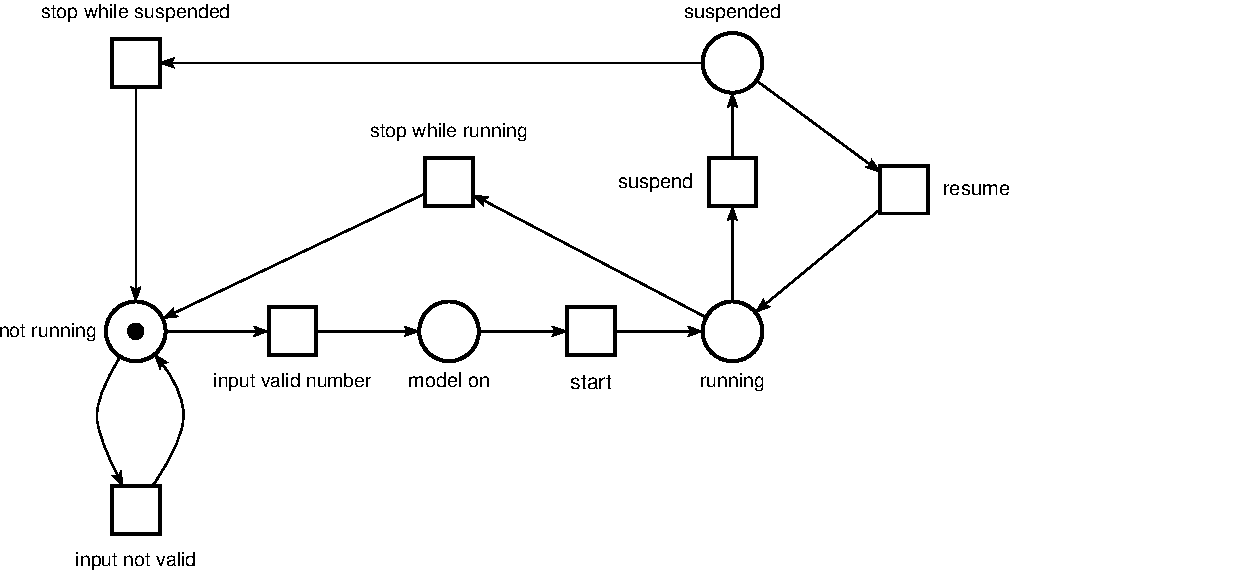
\includegraphics[width=\textwidth]{rete_app_flow.pdf}
    \caption{Rete di Petri per il flusso di esecuzione con input dell'utente.}
    \label{fig:rete_app_flow}
\end{figure}

Per chiarire il comportamento del comando di stop nella rete di Petri mostrata in Fig. \ref{fig:rete_app_flow}, è importante sottolineare che l'evento di stop interrompe immediatamente l'esecuzione dei thread attivi, senza attendere il completamento del ciclo di calcolo corrente.

Questo comportamento è intenzionale e riflette l'implementazione del sistema, dove il comando di stop ha priorità assoluta e causa la terminazione immediata di tutti i thread di simulazione, indipendentemente dal loro stato di avanzamento nel ciclo di calcolo

\section{Ciclo update}
Il ciclo di aggiornamento della simulazione inizia con lo stato iniziale \texttt{start}, seguito dalla fase di calcolo delle velocità (\texttt{update velocity}) eseguita in parallelo da thread distinti (nella figura due). Una volta completato il calcolo, i thread raggiungono una barriera di sincronizzazione (\texttt{velocity barrier}), che garantisce che tutte le velocità siano state aggiornate prima di procedere.

Successivamente, i thread entrano nella fase di aggiornamento delle posizioni (\texttt{update position}), anch'essa eseguita in parallelo. Anche in questo caso, una barriera di sincronizzazione (\texttt{position barrier}) assicura che tutte le posizioni siano state aggiornate correttamente prima di tornare allo stato iniziale, completando così un ciclo di aggiornamento.

Questa rete evidenzia chiaramente i punti di sincronizzazione necessari per mantenere la coerenza del modello, garantendo che le operazioni di calcolo delle velocità e aggiornamento delle posizioni siano eseguite in modo sequenziale e coordinato tra i thread.

\begin{figure}[h!]
    \centering
    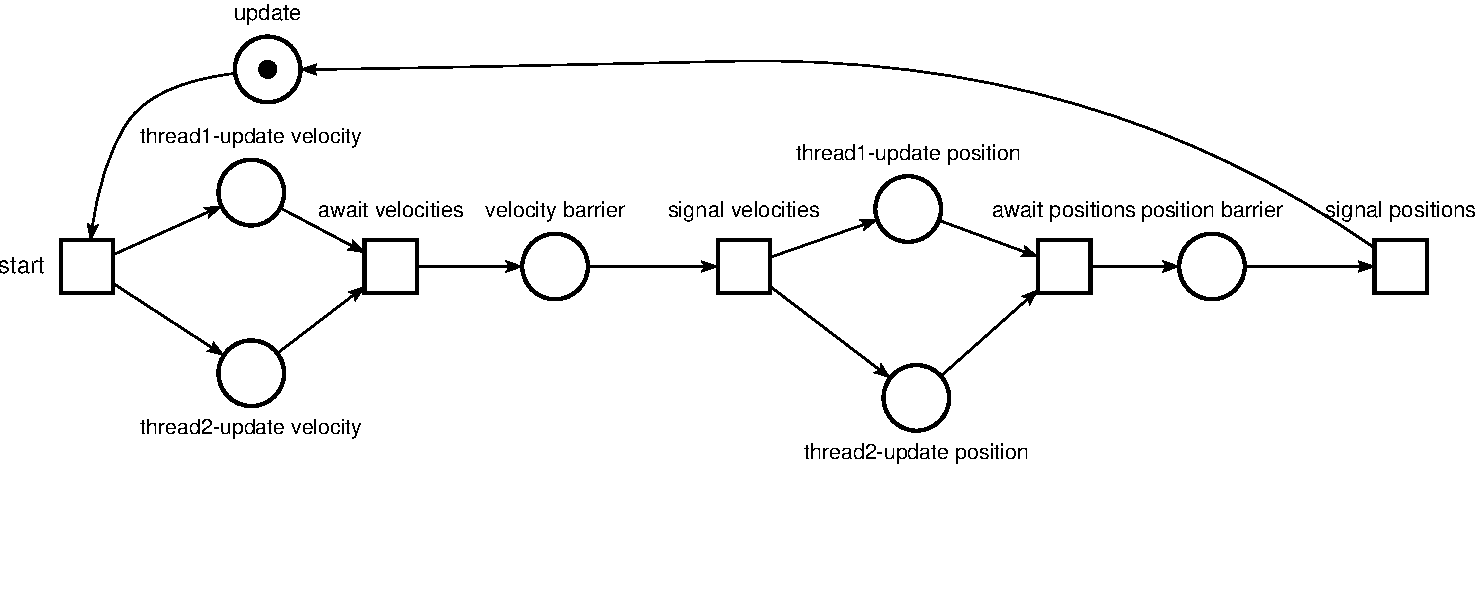
\includegraphics[width=0.8\textwidth]{rete_update_cycle.pdf}
    \caption{Rete di Petri per il ciclo di aggiornamento della simulazione.}
    \label{fig:rete_update_cycle}
\end{figure}

\chapter{Test di performance}
% Performance tests, to analyse and discuss the performance of the programs (for each version) compared to the sequential version
Per valutare l'efficacia delle diverse implementazioni, sono stati condotti test di performance strutturati su diversi scenari e parametri di simulazione. I test sono stati eseguiti su una macchina con [n core] e hanno comparato le quattro versioni dell'algoritmo: sequenziale, platform threads, executor framework e virtual threads.

\section{Metodologia}
I test sono stati condotti con la seguente metodologia:
\begin{itemize}
    \item Numero di boid testati: 500, 1500, 3000
    \item Numero di iterazioni per ciascun test: 100
    \item Metriche raccolte: tempo di esecuzione medio per iterazione (in millisecondi) 
    \item Numero di ripetizioni per test: 3 per garantire significatività statistica (ne riportiamo la media)
\end{itemize}

Per la versione multithreaded tradizionale, sono stati testati diversi numeri di thread (2, 4, 8) per valutare l'impatto del numero di core disponibili. La scelta di questi valori è stata guidata dalla disponibilità di unità di elaborazione fisiche nel sistema di test(massimo 8 core).

La versione Executor e Virtual non è stato testato il cambiamento in base al numero di core, ma piuttosto:
\begin{itemize}
    \item (Executor) il numero di boid assegnato ad ogni task: 1, 50, 300
    \item (Virtual) il numero di boid assegnato ad ogni virtual thread: 1, 50, 300
\end{itemize}

\section{Risultati}

\begin{table}[h!]
    \centering
    \begin{tabular}{|c|c|}
    \hline
    \multicolumn{2}{|c|}{\textbf{Sequential}} \\
    \hline
    \textbf{Boids}& \textbf{Time (ms)}\\
    \hline
    3000 & 6549 \\
    1500 & 1879  \\
    500  & 1163  \\
    \hline
    \end{tabular}
    \caption{Risultati delle performance per configurazioni Sequential}
    \label{tab:sequential-performance}
\end{table}

\begin{table}[h!]
    \centering
    \begin{tabular}{|c|c|c|}
    \hline
    \multicolumn{3}{|c|}{\textbf{Platform}} \\
    \hline
    \textbf{Boids} & \textbf{N threads} & \textbf{Time (ms)}\\
    \hline
    3000 & 8 & 2931 \\
    1500 & 8 & 673  \\
    500  & 8 & 142  \\
    \hline
    \hline
    3000 & 4 & 3266 \\
    1500 & 4 & 802  \\
    500  & 4 & 136  \\
    \hline
    \hline
    3000 & 2 & 4381 \\
    1500 & 2 & 1489  \\
    500  & 2 & 259  \\
    \hline
    \end{tabular}
    \caption{Risultati delle performance per configurazioni Platform}
    \label{tab:platform-performance}
\end{table}

\begin{table}[h!]
    \centering
    \begin{tabular}{|c|c|c|c|}
    \hline
    \multicolumn{4}{|c|}{\textbf{Executor}} \\
    \hline
    \textbf{Boids} & \textbf{Boids/task} & \textbf{Cores} & \textbf{Time (ms)}\\
    \hline
    3000 & 300 & 8 & 13822 \\
    1500 & 300 & 8 & 4614 \\
    500  & 300 & 8 & 1484 \\
    \hline
    \hline
    3000 & 50  & 8 & 15688 \\
    1500 & 50  & 8 & 3841 \\
    500  & 50  & 8 & 1846 \\
    \hline
    \hline
    3000 & 1   & 8 & 27537 \\
    1500 & 1   & 8 & 10132 \\
    500  & 1   & 8 & 2718 \\
    \hline
    \end{tabular}
    \caption{Risultati delle performance per configurazioni Executor}
    \label{tab:executor-performance}
\end{table}

\begin{table}[h!]
    \centering
    \begin{tabular}{|c|c|c|c|}
    \hline
    \multicolumn{4}{|c|}{\textbf{Virtual}} \\
    \hline
    \textbf{Boids} & \textbf{Virtual/task} & \textbf{Cores} & \textbf{Time (ms)}\\
    \hline
    3000 & 300 & 8  & 2381 \\
    1500 & 300 & 8  & 679  \\
    500  & 300 & 8  & 186  \\
    \hline
    \hline
    3000 & 50  & 8  & 2392 \\
    1500 & 50  & 8  & 644  \\
    500  & 50  & 8  & 118  \\
    \hline
    \hline
    3000 & 1   & 8  & 3548 \\
    1500 & 1   & 8  & 849  \\
    500  & 1   & 8  & 207  \\
    \hline
    \end{tabular}
    \caption{Risultati delle performance per configurazioni Virtual}
    \label{tab:virtual-performance}
\end{table}

\newpage

\section{Analisi Comparativa}
Grafico di confronto delle prestazioni
\begin{figure}[H]
    \centering
    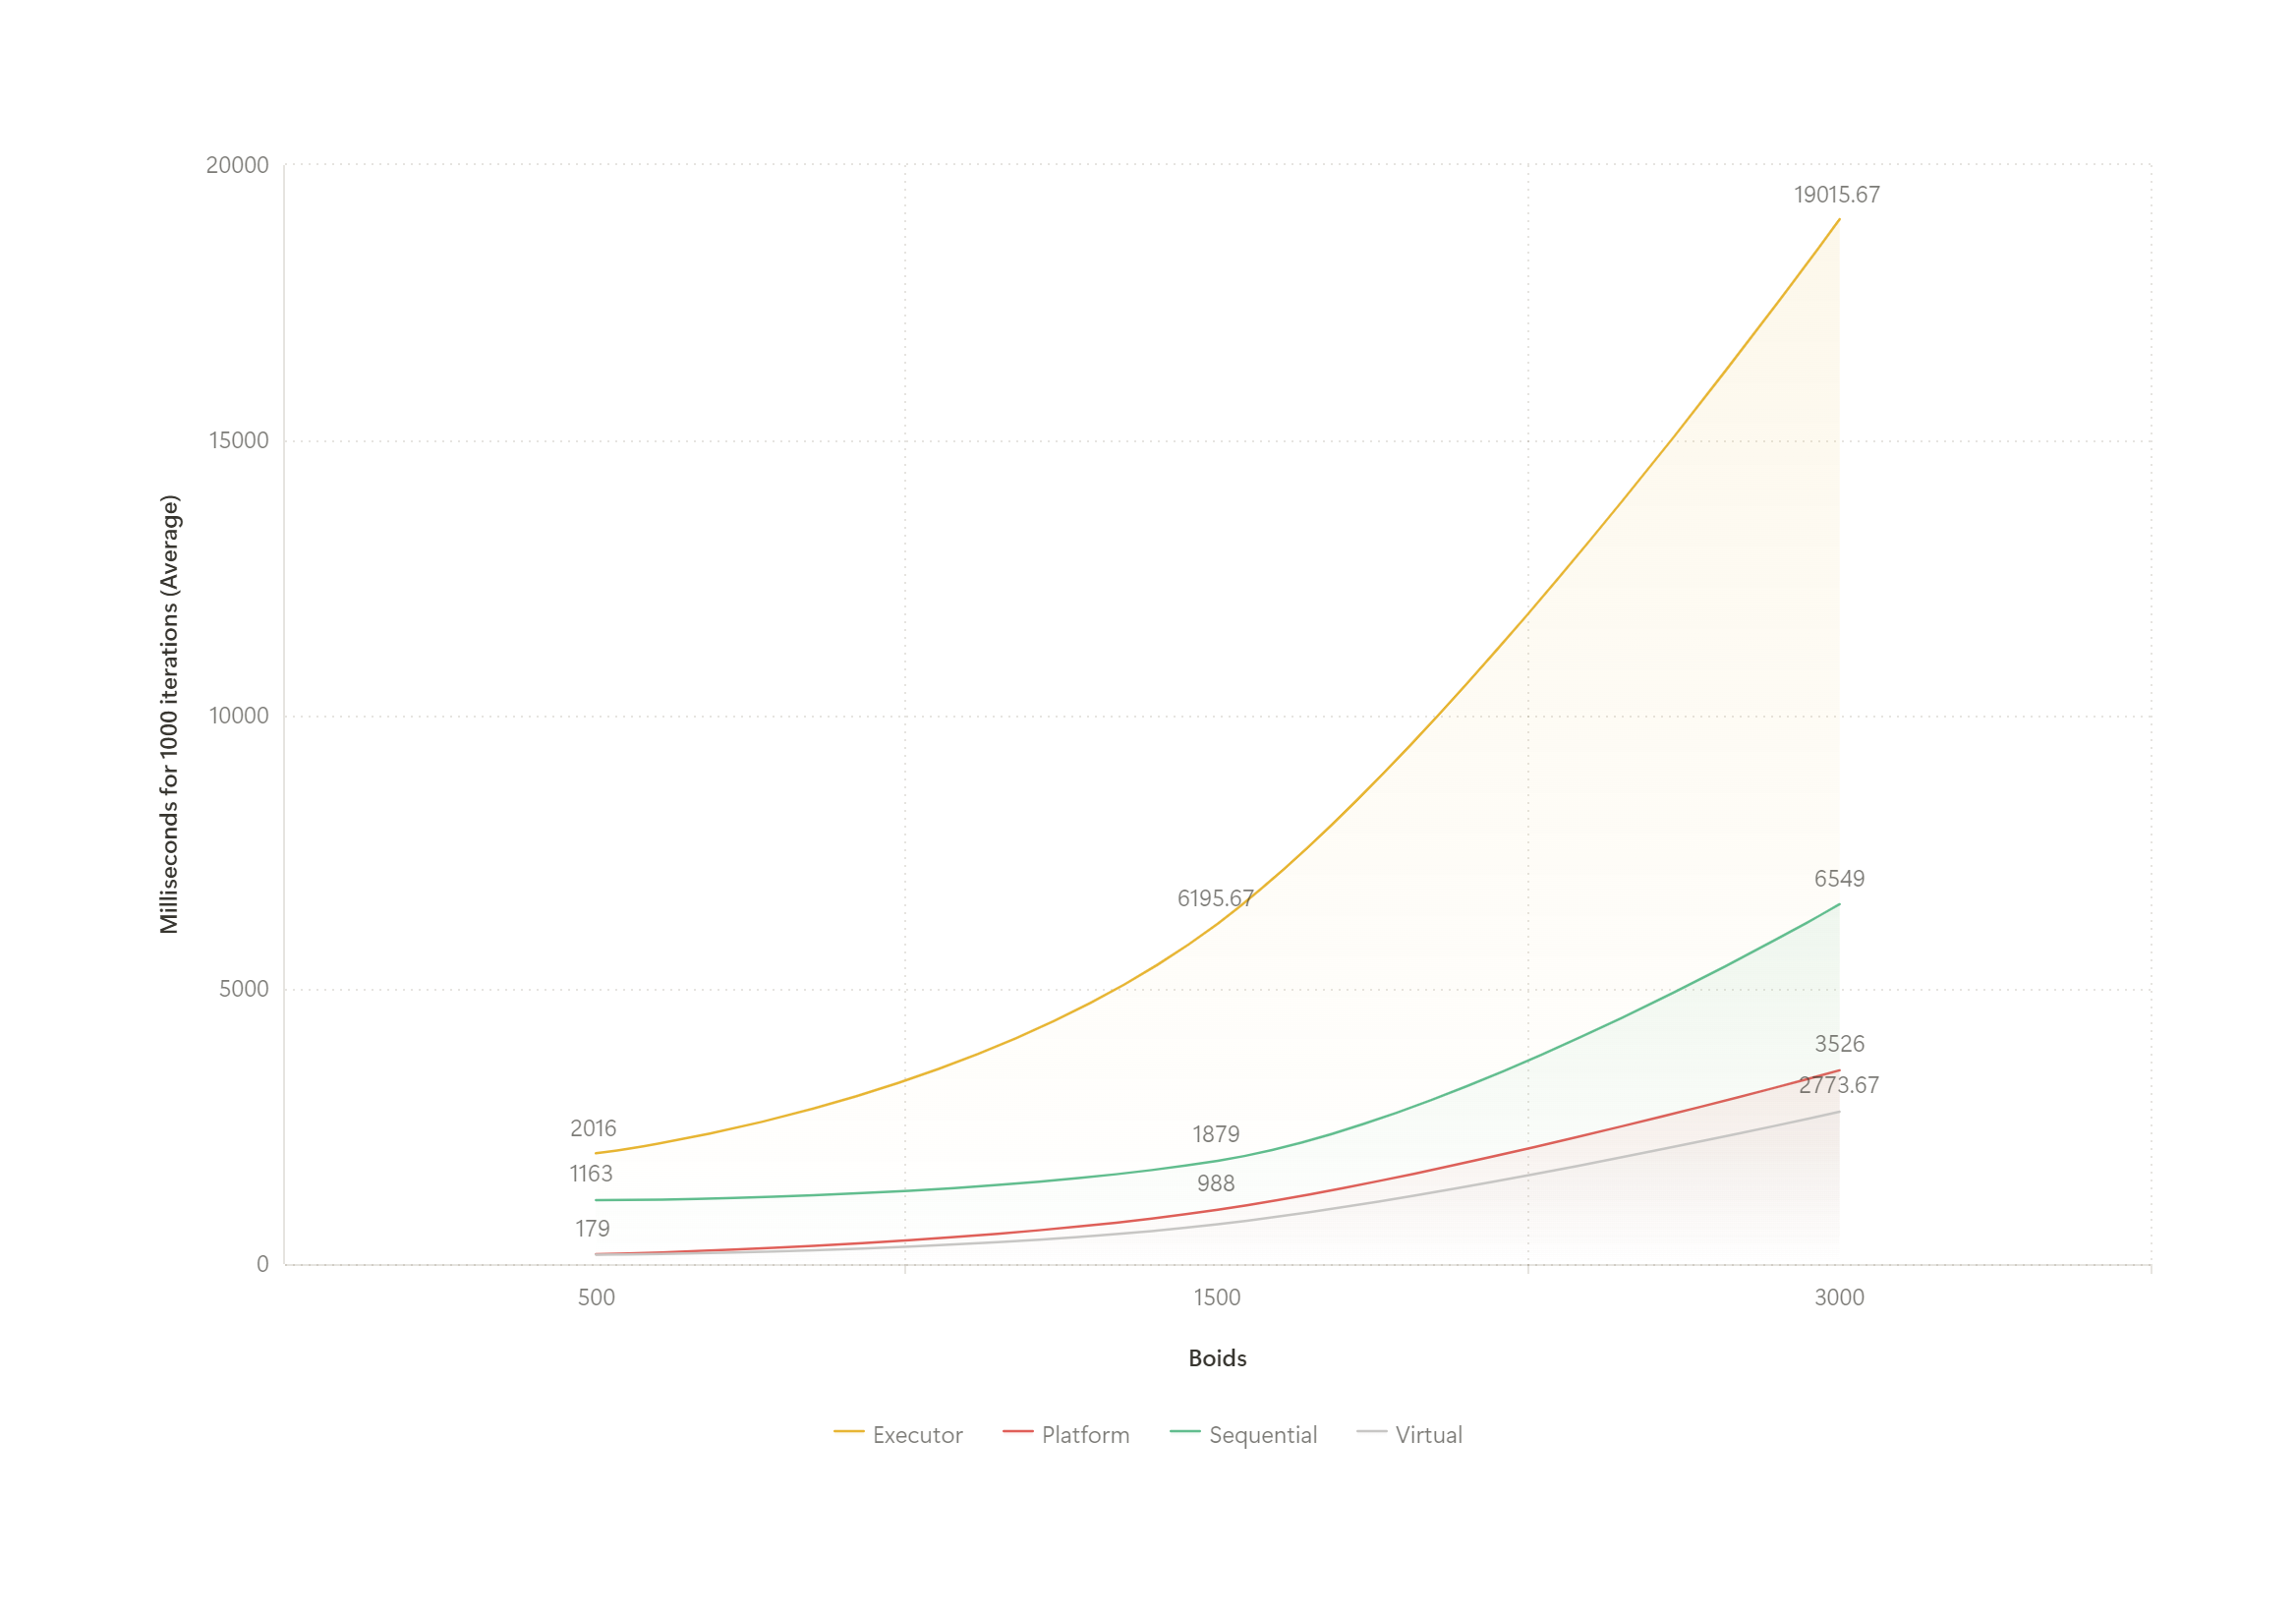
\includegraphics[width=\textwidth]{img/performance_graph.png}
    \caption{Comparazione del framerate medio tra le quattro implementazioni al variare del numero di boid.}
    \label{fig:performance_comparison}
\end{figure}

La misura quantitativa delle prestazioni nella programmazione concorrente è lo \textbf{speedup}, definito come:

\[
S = \frac{T_1}{T_N}
\]

dove:
\begin{itemize}
    \item $N$ è il numero di processori
    \item $T_1$ è il tempo di esecuzione dell'algoritmo sequenziale
    \item $T_N$ è il tempo di esecuzione dell'algoritmo parallelo con $N$ processori
\end{itemize}

\begin{table}[h!]
    \centering
    \begin{tabular}{|c|c|c|c|}
    \hline
    \textbf{Boids}& \textbf{Sequential (ms)}& \textbf{Platform (ms)} & \textbf{Speed-up} \\
    \hline
    500  & 1163 & 142 & 8.19  \\
    1500 & 1879 & 673 & 2.79  \\
    3000 & 6549 & 2931 & 2.23 \\
    \hline
    \end{tabular}
    \caption{Risultati calcolo speedup per configurazioni Platform}

    \label{tab:platform-speedup}
\end{table}

I risultati evidenziano pattern significativi nelle performance delle diverse implementazioni:

\begin{itemize}
    \item L'implementazione con platform threads mostra un sostanziale miglioramento rispetto alla versione sequenziale, con prestazioni che migliorano all'aumentare dei thread fino a saturare il numero di core fisici disponibili.
    
    \item L'implementazione basata su Executor Framework presenta un overhead computazionale considerevole, risultando la meno efficiente tra le soluzioni testate. Questo overhead può essere attribuito alla gestione dei numerosi task e alla sincronizzazione basata sui Future, che introduce un costo aggiuntivo rispetto alla sincronizzazione diretta con barriere.
    
    \item L'implementazione con virtual threads emerge come la soluzione più efficiente, offrendo prestazioni paragonabili o leggermente superiori all'implementazione con platform threads, ma con una complessità implementativa inferiore. La leggerezza dei virtual thread consente di ottenere un elevato grado di parallelismo con un overhead ridotto.
\end{itemize}

È interessante notare come la granularità della parallelizzazione influenzi le prestazioni: nella versione Virtual, la configurazioni con 50 boid per unità di lavoro tende a offrire il miglior compromesso tra overhead di gestione e utilizzo efficiente delle risorse di calcolo.


\chapter{Verifica con JPF}
% Verification of the program (a model of it) using JPF. For this point, only the Java multithreaded programming version may be considered.
In questa sezione viene discussa la verifica formale dell'implementazione multi-thread dell'algoritmo dei boid utilizzando Java PathFinder (JPF), uno strumento di model checking sviluppato dalla NASA per analizzare programmi Java. 
JPF è particolarmente utile per verificare le proprietà di sicurezza e correttezza in sistemi concorrenti, individuando problematiche tipiche della programmazione parallela.

L'analisi si è concentrata su una versione semplificata del modello, mantenendo gli aspetti essenziali di sincronizzazione tra i thread attraverso la nostra implementazione personalizzata `MyBarrier`. La verifica ha l'obiettivo di garantire l'assenza di deadlock e la corretta sincronizzazione tra le fasi di calcolo delle velocità e aggiornamento delle posizioni evitando corse critiche, elementi fondamentali per la correttezza dell'algoritmo.

\section{Scorporazione del modello}
Per diminuire il numero di stati esplorati da JPF, è stato necessario semplificare il modello originale. La versione semplificata mantiene la logica di calcolo delle velocità e aggiornamento delle posizioni, ma elimina le interazioni con l'interfaccia grafica e altre funzionalità non essenziali per la verifica formale.

In particolare sono state rimosse le seguenti componenti:
\begin{itemize}
    \item tutta la View, che gestiva l'interfaccia grafica e il rendering dei boids
    \item il controllo di flusso con \texttt{start}, \texttt{stop}, \texttt{suspend} e \texttt{resume} 
    \item randomicità nella generazione delle posizioni iniziali e velocità dei boids, perchè altrimenti JPF avrebbe esplorato tutti i possibili valori nel range di quelli casuali
    \item il numero di boids, abbassato e fissato a 5
    \item il numero di thread, fissato a 2
\end{itemize}

Inoltre è stato necessario reimplementare come classi \texttt{P2d} e \texttt{V2d} che erano stati progettati come record, costrutto introdotto in Java 21, perchè JPF compila invece con Java 11 al massimo, dunque non sono supportati.

\section{Risultati}

\subsection{Corsa critica in MyBarrier}
La verifica con JPF ha permesso di individuare una corsa critica che si verificava quando i thread si risvegliavano dopo aver raggiunto la barriera di sincronizzazione.

\begin{verbatim}
====================================================== error 1
gov.nasa.jpf.listener.PreciseRaceDetector
race for field pcd.ass01.MyBarrier@250.broken
    Thread-1 at pcd.ass01.MyBarrier.reset(MyBarrier.java:53)
        "broken = false;"  
        WRITE: putfield pcd.ass01.MyBarrier.broken
    Thread-2 at pcd.ass01.MyBarrier.reset(MyBarrier.java:52)
        "if (broken) {"  
        READ:  getfield pcd.ass01.MyBarrier.broken
====================================================== 
\end{verbatim}

La verifica ha identificato una corsa critica nella classe \texttt{MyBarrier}: quando i thread si risvegliavano dopo aver raggiunto la sincronizzazione, accedevano contemporaneamente alla variabile condivisa \texttt{broken} senza adeguata protezione. In particolare, alcuni thread potevano leggere questa variabile mentre altri la stavano modificando.

Il problema è stato risolto estendendo la sezione critica nel metodo \texttt{reset} mediante un lock che garantisce l'accesso esclusivo durante il reset della barriera, assicurando che la reinizializzazione dello stato della barriera avvenga in modo atomico e coerente tra i thread partecipanti.

\subsection{Corsa critica in updateVelocity}
Risolvendo il problema precedente, JPF ha evidenziato un'ulteriore criticità.

\begin{verbatim}
====================================================== error 1
gov.nasa.jpf.listener.PreciseRaceDetector
race for field pcd.ass01.Boid@230.vel
    Thread-1 at pcd.ass01.Boid.updateVelocity(Boid.java:39)
        ".sum(cohesion.mul(model.getCohesionWeight()));"  
        WRITE: putfield pcd.ass01.Boid.vel
    Thread-2 at pcd.ass01.Boid.getVel(Boid.java:23)
        "var value = vel;"  
        READ:  getfield pcd.ass01.Boid.vel
======================================================
\end{verbatim}

Durante l'esecuzione del metodo \texttt{updateVelocity} infatti, ogni thread accede in lettura all'intero insieme dei boid per calcolare le forze di coesione, separazione e allineamento, mentre modifica il campo \texttt{velocity} del boid corrente. Questa situazione genera una corsa critica quando un thread legge la velocità di un boid che viene contemporaneamente modificata da un altro thread.

In particolare, se due thread accedono a boid diversi, ma uno di questi boid ha il campo \texttt{velocity} modificato da un altro thread, si verifica una race condition. Per affrontare questo problema, sono state esplorate due soluzioni principali:

\begin{itemize}
    \item \textbf{Copia difensiva:} Ogni thread lavora su una copia locale dei boid, che viene poi utilizzata per sovrascrivere i boid originali al termine del calcolo delle nuove velocità e posizioni. Tuttavia, questa soluzione ha introdotto problemi di coerenza, rompendo l'algoritmo di simulazione nell'applicazione principale.
    \item \textbf{Lock sul campo \texttt{velocity}:} È stato implementato un meccanismo di lock per proteggere l'accesso al campo \texttt{velocity} del boid corrente. Questo approccio ha garantito che ogni thread potesse accedere e modificare la velocità di un boid senza interferenze da parte di altri thread, preservando la correttezza dell'algoritmo.
\end{itemize}

La soluzione basata sul lock si è dimostrata efficace, eliminando le corse critiche e mantenendo il comportamento corretto dell'algoritmo. Sebbene l'uso di lock possa introdurre un leggero overhead, esso è stato ritenuto accettabile rispetto ai benefici in termini di affidabilità e coerenza del sistema.

\begin{verbatim}
====================================================== system under test
pcd.ass01.BoidsSimulation.main()

====================================================== search started: 00:03
====================================================== results
no errors detected

====================================================== statistics
elapsed time:       00:01:17
states:             new=235051,visited=349268,backtracked=584319,end=0
search:             maxDepth=2073,constraints=0
choice generators:  
    thread=235052 
    (signal=0,lock=1111,sharedRef=211717,threadApi=4,reschedule=19710)
    data=0
heap:               new=142192,released=249301,maxLive=763,gcCycles=571041
instructions:       22882466
max memory:         364MB
loaded code:        classes=127,methods=3161

====================================================== search finished: 00:04
\end{verbatim}

\end{document}
